\documentclass[aps,pre,12pt,preprint,%
	onecolumn,showpacs,showkeys,nofootinbib]{revtex4-1}
%Chinese
	\usepackage[UTF8,fontset=fandol]{ctex}
	\xeCJKsetup{underdot = {
		boxdepth=0pt, format=\huge, depth=.4em
	}}
%	\usepackage[datesep=/]{datetime2} % Use default
	\DeclareTextFontCommand{\textbf}{\sffamily}
%Presenting
	\usepackage[table]{xcolor}
	\usepackage{graphicx}
	\usepackage[space]{grffile}
	\usepackage[font=small,format=plain,%
		labelfont=bf,textfont=it,%
		singlelinecheck=false]{caption}
	\usepackage[above]{placeins}
%	\usepackage{float} % Cause trouble for table footnotes
	\usepackage{wrapfig}
	\usepackage{tabularx,array,booktabs,multirow,bigstrut}
	\newcolumntype{C}[1]{>{\hsize=#1\hsize%
		\centering\arraybackslash}X}
	\newcommand{\minitab}[2][l]{%
		\begin{tabular}{#1}#2\end{tabular}}
	\usepackage{setspace,dcolumn}
	\usepackage{subfig}
	\usepackage{psfrag,epsfig}
%MathSetting
	\let\latexointop\ointop
	\usepackage{amsmath,bm,amssymb,esint,extarrows}
	\usepackage{upgreek,textcomp,mathrsfs}
	\usepackage[only,sslash]{stmaryrd}
	\usepackage{nicefrac,eqnarray}
%	\usepackage{amsthm} % Enable when necessary
%	\usepackage[mathscr]{eucal} % Enable when necessary
	\usepackage{mathtools,physics,siunitx}
	\usepackage{stackengine,varwidth}
	\usepackage{tikz}
	\usepackage{resizegather,empheq}
	\usetagform{default}
	\usepackage{calligra,fourier-orns}
	% Keep \oint unchanged by esint
	\let\ointop\undefined
	\let\ointop\latexointop
	% Define a scriptr 
	\DeclareMathAlphabet{\mathcalligra}{T1}{calligra}{m}{n}
	\DeclareFontShape{T1}{calligra}{m}{n}{<->s*[2.2]callig15}{}
	\newcommand{\scriptr}{\mathcalligra{r}\,}
	\newcommand{\rvector}{\pmb{\mathcalligra{r}}\,}
	% Useful shorthand
	\DeclarePairedDelimiter\ave{\langle}{\rangle}
	\newcommand\inlineeqno{\stepcounter{equation}\ (\theequation)}
	\newcommand{\sinc}{\operatorname{sinc}}
	\newcommand{\mbb}[1]{\mathbb{#1}}
	\newcommand{\mrm}[1]{\mathrm{#1}}
	\newcommand{\mcal}[1]{\mathcal{#1}}
	\newcommand{\tup}[1]{\textup{#1}}
	% Scaling and positioning
	\newcommand\scalemath[2]{\scalebox{#1}{\mbox{\ensuremath{\displaystyle #2}}}}
	\newcommand\raisemath[2]{\raisebox{#1\depth}{${#2}$}}
	\empheqset{box=\nicebox}
	% Presenting
	\newcommand*\nicebox[1]{\fbox{\hspace{1em}\addstackgap[5pt]{#1}\hspace{1em}}}
	\sisetup{%
		redefine-symbols=false,%
		separate-uncertainty=true,%
		range-phrase=\,\textasciitilde\,,%
		arc-separator = \,}
	\allowdisplaybreaks[2]
%ParagraphSetting
	\setlength{\parskip}{.3\baselineskip}
	\usepackage[defaultlines=2,all]{nowidow}
	\postdisplaypenalty=50
%PageSetting
	\usepackage{titlesec}
	\titleformat*{\section}{\large\bfseries}
	\usepackage[colorlinks=true,linkcolor=blue]{hyperref}
	\newcommand{\texstringonly}[1]{%
		\texorpdfstring{#1}{}}
	\usepackage[vmargin={3.5cm,4cm},hmargin=3cm,%
		footnotesep=\baselineskip]{geometry}
%	\usepackage[bottom]{footmisc} % Cause trouble for table footnotes
	\usepackage{changepage}
	% Autoref names
	\renewcommand{\tableautorefname}{\tablename}
	\renewcommand{\figureautorefname}{\figurename}
	% List settings
	\usepackage{enumitem}
	\setlist{itemsep=0pt,topsep=0pt,labelindent=\parindent,leftmargin=0pt,itemindent=*}
	% Some redefined lengths
	\setlength{\headsep}{1.6\baselineskip}
%	\setlength{\footnotesep}{3\parskip} % Use when necessary
	% Header
	\usepackage{fancyhdr,lastpage}
	\pagestyle{fancy}
%	\fancyhf{} % Clear default settings; disabled for now
	\cfoot{--\ \thepage\,/\,\pageref{LastPage} \ --}
	\setlength{\footskip}{2\baselineskip}
	\renewcommand{\headrulewidth}{0.1pt}
	\renewcommand{\headrule}{
		\ifnum\value{page}=1\relax\else
			\vbox to 2pt{
			\hbox to \headwidth{\dotfill}\vss}
		\fi}
	\fancypagestyle{titlepagestyle}{%
		\fancyhead{}
		\chead{
			\vspace{2.5\baselineskip}
			
\includegraphics[width=.75\linewidth]{../PKUPhy}}
	}
	% Separator
	\newcommand{\newparagraph}{\pagebreak[3]\noindent%
		\hfil
		~\raisebox{-4pt}[10pt][10pt]{\decofourright~~~~~~~~\decofourleft}~ %
		\par
	}
%	% Background % Use when necessary
%	\usepackage{background} %Waterstamp package
%	\SetBgContents{...的实验报告} %Waterstamp to prevent copying
%	\SetBgScale{5} %Waterstamp setting
	% Essay format
	\renewcommand\appendixname{附录}
	\renewcommand\abstractname{}%摘要
	\renewcommand\tablename{表}
	\renewcommand\figurename{图}
	\renewcommand\refname{参考文献}
	\makeatletter
	\def\@pacs@name{\songti\zihao{-4}{\bf PACS码:}}
	\def\@keys@name{\songti\zihao{-4}{\bf 关键词:}}
	\def\Dated@name{日期:}
	\def\Received@name{\zihao{-5}{接收} }
	\def\Revised@name{\zihao{-5}{修订} }
	\def\Accepted@name{\zihao{-5}{采纳} }
	\def\Published@name{\zihao{-5}{发表} }
	\makeatother
	\linespread{1.5}
	\renewcommand{\labelenumi}{\alph{enumi}.}
	\leftmargini=20mm
	\newcommand{\supercite}[1]{\textsuperscript{\,%
		[\citenum{#1}]}}
	\let\fancycite\cite
	\renewcommand{\cite}[1]{\textup{\fancycite{#1}}}
	% Math line spacing
	\newlength{\djot}
	\setlength{\djot}{\jot}
	\newcommand{\restorejot}{\setlength{\jot}{\djot}}

%Miscellaneous
%	\newcommand{\tabindent}{\hspace{2em}}
%FourierTransform
	\newcommand{\fourierf}{\mathscr F}
%Atoms
	\newcommand{\SrAtom}{\,\textsuperscript{90}\tup{Sr}\,}
	\newcommand{\Yatom}{\,\textsuperscript{90}\tup{Y}\,}
	\newcommand{\CsAtom}{\,\textsuperscript{137}\tup{Cs}\,}
	\newcommand{\CoAtom}{\,\textsuperscript{60}\tup{Cs}\,}
\begin{document}
%Basic Data
	\title{%
	\texstringonly{\hfil\\[2\baselineskip]}
	\sf\LARGE%
		用\texorpdfstring{$\beta$}{β}粒子检验相对论性动量--动能关系%
	\texstringonly{\vspace{3ex}}}
	\author{\fangsong\large%
		Bryan%
	\vspace{2mm}}
	\affiliation{\it%
		北京大学物理学院~~学号:\normalfont 1500000000\,}
	\date{\today}
	\keywords{狭义相对论,色散关系,$\beta$衰变,$\beta$粒子}
	\email{guesswhat@email.addr;}

\begin{abstract}
\vspace{10mm}
\begin{spacing}{1.5}\normalsize
\setlength{\parskip}{.3\baselineskip}
%	200—300字,
%	说明用什么方法做了什么事,
%	由此得到什么结果和结论,
%	有何意义.
%	不用缩略词,不用第一人称.
%%%%%%%%%%%%%%%%%%%%%%%%%%%%%%%%
	对于高速运动的物体,狭义相对论给出了与经典情形完全不同的描述;本实验旨在从动量--能量关系这一角度,验证这一描述的准确性。实验中使用\SrAtom--\Yatom\,$\beta$源产生速度接近光速的$\beta$粒子,通过分别测定其动量、能量,分析其动量--能量关系,验证了狭义相对论的预测。
	
	在此基础上,本实验进一步探究了空气对$\beta$粒子运动的影响;证实了空气导致$\beta$粒子的自由程显著减小,并对 \SI{1}{atm} 下$\beta$粒子的衰减长度进行了估计。这确认了真空环境在本实验中的必要性。
\end{spacing}
\end{abstract}

\maketitle
\thispagestyle{titlepagestyle}

%	\item 课程实验报告应假定读者既不是已知全部实验细节的指导教师,也不是缺少专业知识的公众,而是同领域的实验研究者,或审稿人. 不能要求读者要在读过课程讲义后才能读懂课程实验报告.
%	\item 公式、图和表要分别用阿拉伯数字编列序号. 公式和图表要达到可发表的质量.
%	\item 凡不是自己独立思考得到的内容都应该引参考文献. 不能大段引用同一参考文献. 对复杂问题,应该优先考虑引用参考文献得到结果. 对简单一些的问题才鼓励独立思考.
%	\item 较长的推导和说明可以作为附件提交,不占用报告篇幅.
%	\item 思考题不是报告的组成部分. 应另起一页附在报告的最后.
\section{引言}
%%	研究论文引言一般包含以下内容:
%%	(1)所研究领域背景和现状;
%%	(2)有待研究的问题;
%%	(3)本研究的目的、主要内容和结果;
%%	(4)结果的意义.\par
%%	在写实验报告的引言时,同学可以假想自己是第一个做类似研究的人.\par
%%	引言一定要切合报告正文,不能漫无目的地介绍背景. 要快速地将读者引导到报告主题上,并作较深入的讨论.\par
%%	引言篇幅可以在较大范围内变化,但最长不应超过报告文字篇幅的1/3.\par
%%	引言撰写可以参考实验讲义,可以复述,但不能复制讲义上的任何一句话.\par
%%%%%%%%%%%%%%%%%%%%%%%%%%%%%%%
	19世纪,电磁理论得到了极大的发展;麦克斯韦(James C. Maxwell)等人的工作表明,电磁理论可以完美地整合到一组方程中\supercite{maxwell1865dynamical},这便是麦克斯韦方程组。麦克斯韦方程组完整地描述了经典电动力学中的现象,其波动解自然地给出了\textit{电磁波}的预测;通过计算波速:
	\begin{equation}
		c = \frac{1}{\sqrt{\epsilon_0\mu_0}}
		\label{eq:lightSpeed}
	\end{equation}
	麦克斯韦发现\supercite{maxwell1865dynamical}, 可见光正是一种电磁波,从而统一了光学和电磁学。
	
	然而,麦克斯韦方程与经典的伽利略变换不可调和。于是人们猜测,麦克斯韦方程实际只适用于一个特殊的参考系;相应地,电磁波在一种特殊的介质——以太(aether)中传播,可以通过精确测量光速的变动获得地面参考系相对以太的漂移速度。然而,实验迹象表明,这一漂移速度十分微小;迈克尔逊--莫雷实验(Michelson–Morley experiment, 1887)\supercite{michelson1887relative} 给出漂移速度的上限为 \SI{8}{\km/\s}, 考虑地球的公转以及太阳系的运动,这一速度实在微乎其微,令人费解\footnote{%
		最近的实验结果给出的上限为$10^{-17}c \approx \SI{3}{\nm/\s}$, 参见 \cite{herrmann2009rotating}. 
	}。
	
	人们不得不转而考虑另一种可能的办法,即对伽利略变换进行修正。经由洛仑兹(Hendrik Lorentz, 参见\cite{lorentz1904electromagnetic})、庞加莱(Henri Poincaré, 参见\cite{poincare1976measure})及爱因斯坦(Albert Einstein)等人的共同努力,以洛仑兹变换为基础的狭义相对论时空观得以建立。相对论时空观与经典时空观的主要差异在于:
	\begin{enumerate}[noitemsep]
	\item \textbf{光速不变:}在所有惯性系中,真空光速恒为$c$, 它同时也是运动速度的上限;
	\item \textbf{相对时空:}不存在绝对时空,尤其是不存在绝对的时间坐标;所有惯性系在物理上都是平等的,物理规律具有相同的形式。\vspace{2ex}
	\end{enumerate}
\pagebreak
	
	\vspace{3ex}
	相对论时空观自然与电动力学相容,但又引出了一些新的疑问。例如,作为时间相对性的直接推论,运动的时钟与静止的时钟并不同步(\textit{钟慢效应});类似的反直观现象还有\textit{动尺收缩}等等。进一步,对于高速运动的粒子而言,狭义相对论的动力学对物体的动量--动能关系做出了不寻常的预计;通过探测高速运动粒子的动量和能量,我们可以方便地验证这一新的\textit{色散关系}(dispersion relation, 借用了光学中动量--能量关系的等价表述),从而初步检验狭义相对论的正确性;此即本实验的首要目的。
\section{理论}
	相对论性的时空由事件(events)构成,时空间隔表示为\textit{四矢量}:
	\begin{equation}
	\begin{gathered}
		\dd{x^\mu} \sim
		\pqty{\begin{smallmatrix}
			c\,\dd{t} \\[1ex] \dd{\vb{x}}
		\end{smallmatrix}},\quad\mu = 0,1,2,3,\\
		\dd{x^0} = c\dd{t}, \quad \dd{x^i} = \dd{\vb{x}^i},\quad
		i=1,2,3
	\end{gathered}
	\end{equation}
	其中$c$为光速;光速不变原理表明,变换到另一惯性系后,相应的\textbf{时空间隔}保持不变(类似于洛仑兹变换中,空间间隔保持不变),即:
	\begin{equation}
	\begin{gathered}
		\eta_{\mu\nu} \dd{x^\mu} \dd{x^\nu}
		\equiv \sum_{\mu,\nu} \eta_{\mu\nu} \dd{x^\mu} \dd{x^\nu}
		= (c\dd{t})^2 - \dd{\vb{x}}^2\ 
		\textit{是洛仑兹不变量(标量),} \\
		\eta_{\mu\nu} \sim
		\pqty{\begin{smallmatrix}
			1 & & & \\
			& -1 & & \\
			& & -1 & \\
			& & & -1
		\end{smallmatrix}}
	\end{gathered}
	\end{equation}
	
	考察运动物体的\textit{共动}参考系,其时间坐标$\tau$称为\textit{固有时}或\textit{原时},有:
	\begin{equation}
	\begin{gathered}
		(c\dd{\tau})^2 - 0 = (c\dd{t})^2 - (\dd{\vb{x}})^2\quad
		\Rightarrow\quad
		\dd{\tau} = \dd{t} \sqrt{1 - \frac{\vb{v}^2}{c^2}}
		= \frac{1}{\gamma}\dd{t},\\
	\end{gathered}
	\end{equation}
	这里$\gamma = \frac{1}{\sqrt{1 - \frac{\vb{v}^2}{c^2}}}$. $\gamma$因子表征了相对论与经典情形的差异。
	\vspace{6ex}
\pagebreak
	
	四动量$p^\mu = m\dv{x^\mu}{\tau} \sim \gamma m
		\pqty{\begin{smallmatrix}
			c \\[1ex] \vb{v}
		\end{smallmatrix}}
		=
		\pqty{\begin{smallmatrix}
			E/c \\[1ex] \vb{p}
		\end{smallmatrix}}$, 它同样是洛仑兹标量;这给出:
	\begin{equation}
	\begin{gathered}
		\eta_{\mu\nu} p^\mu p^\nu
		= \pqty{\frac{E}{c}}^2 - \vb{p}^2 = (mc)^2,\\
		E^2 = \vb{p}^2 c^2 + m^2 c^4
		\label{eq:E-Prelations}
	\end{gathered}
	\end{equation}
	此即相对论性色散关系。我们发现,非零质量的粒子不仅具有动能,还具有\textit{静能}$mc^2$; 扣除掉静能后,粒子的动能可表示为:
	\begin{equation}
		E_k = \sqrt{p^2 c^2 + m^2 c^4} - m^2 c^4
		\,\to\, \frac{1}{2} mv^2 \pqty{
			1 + \mcal{O}\,\pqty{\frac{v}{c}}^2
		}
	\label{eq:relativityEk}
	\end{equation}
	
	可见,在低速极限下,相对论性色散关系回归至经典情形;而对于高速运动的粒子,$\pqty{\frac{v}{c}}^2$阶项不可忽略,两者将会出现显著的差异。本实验即采用$\beta$衰变产生的高速$\beta$粒子,试图观测这一非经典的现象。
\section{实验装置}
%%	在此部分需要将实验条件交待清楚到别人能重复你的实验结果的程度. 此外,还需表明你已尽了最大努力来提高实验精度和结果的可靠性. 简单的不确定度估计可以在此节给出,复杂一些的可以放到分析讨论部分.\par
%%	实验条件不仅是指直接影响实验结果的实验参量,而且还包括影响实验质量和可靠性的因素,如室温、空气湿度、基真空、原材料纯度等.\par
%%	作为教学实验报告,此节写详细一点没有坏处.\par
%%	成段有叙述,必要才分节。
%%%%%%%%%%%%%%%%%%%%%%%%%%%%%%%
	实验装置的基本结构如图 \ref{fig:app} 所示,
	使用\SrAtom--\Yatom\,$\beta$源产生高速$\beta$粒子(负电子,质量$m = \SI{.511}{\MeV/c^2}$),能量上限为 \SI{2.27}{\MeV}, 假定相对论色散关系确切无误,这意味着粒子的速度最高可达 97\% 光速,应当出现显著的相对论效应。
	
	带电粒子的动量通过\textbf{磁谱仪}测定。据经典电动力学,磁场中电子的运动方程:
	\begin{equation}
		\dv{\vb{p}}{t} = -e\vb{v}\times\vb{B}
	\end{equation}
	注意到相对论与电动力学的相容性,此运动方程对高速情形依然成立;垂直射入匀强磁场中的粒子轨迹为圆弧,方程进一步简化为:
	\begin{equation}
		p = eBR = \pqty{\frac{BRc}{\si{M\V}}} \frac{\si{\MeV}}{c}
	\end{equation}
	
	\begin{figure}[!h]
	\vspace{-3ex}
	\centering
	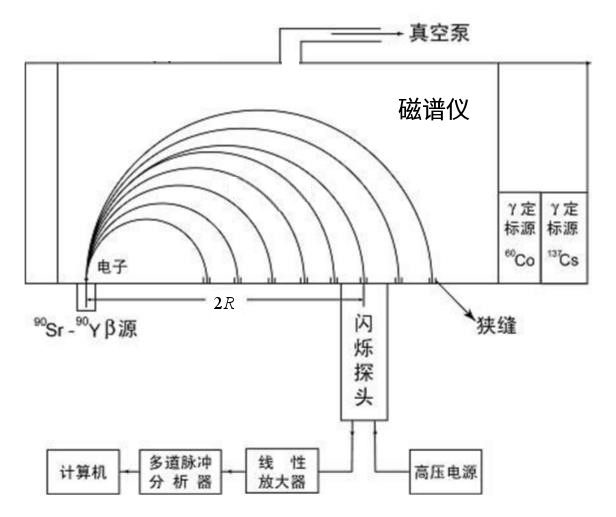
\includegraphics[width=.6\linewidth]{app+.png}
	\caption[装置]{实验装置示意图,参考\cite{textbook}. 
		\vspace{-.5ex}}
	\raggedright\small
	\textit{\hphantom{说明}
		$\beta$粒子源出射的粒子经准直后进入磁谱仪,
		真空泵可控制其真空度,减少碰撞导致的能动量改变。
		$\beta$粒子运动半周后离开磁谱仪,进入闪烁探头;
		数据按图示流程进行采集、分析。闪烁探头固定在轨道上,有坐标$x$便于确定其位置;实际有:\vspace{-1.2ex}
		\[2R = x - \SI{6.15}{\cm}\]}
	\vspace{-2ex}
	\label{fig:app}
	\end{figure}
	
	应当注意,辐射阻尼可能导致粒子损失动能。利用亚伯拉罕--洛仑兹方程:
	\begin{equation}
		\vb{F} = \frac{e^2}{6\pi\epsilon_0 c^3} \dot{\vb{a}}
	\end{equation}
	结合本实验中装置的$B = \SI{603.4}{G} = \SI{60.34}{\milli\tesla}$, 加速度的变化率$\dot{a} \sim \frac{v^2}{r} \cdot \frac{v}{r}$, 估计辐射阻尼的等效作用力$F$及外磁场作用力$evB$分别为:
	\begin{equation}
		F \sim \frac{e^2}{6\pi\epsilon_0 r^2}
			\pqty{\frac{v}{c}}^3
			\sim \SI{e-26}{\N},\quad
		evB \sim ecB \pqty{\frac{v}{c}}
			\sim \SI{e-12}{\N}
	\end{equation}
	因此可以安全地略去辐射阻尼的影响。
	
	动能测定通过 NaI (Tl) \textbf{闪烁体探测器}实现。入射粒子的动能传递给闪烁体使之激发、退激,放出光子(\textit{闪烁}),经光电倍增、前置放大、线性放大等步骤,转化为充分强的电脉冲输入\textbf{多道分析器};多道分析器将脉冲强度转化为道址$n$存储并计数。
	
	本实验中,光电倍增管加高压$U = \SI{594}{\V}$. 注意,上述能量转换过程基本上是线性的,即有$n\propto E$; 利用标准放射源\CsAtom 和\CoAtom 进行定标,可进一步确定$n$--$E$关系,由此获得粒子的动能。此外,$\beta$粒子在穿入、穿出真空室以及进入探头的过程中存在能量损失,需要进行修正;采用 \cite{textbook} 给出的数值进行修正\footnote{%
		参考\cite{textbook} p.\numrange{96}{97}, 表2-6-1及2-6-2. }。
\section{结果与分析}
%	实验结果应尽量以图表的形式给出. 每一个图表都应该是完整的,即阅读图表时可以不必依赖正文.\par
%	依自己意愿,实验结果和对结果的分析讨论既可分为两节也可合在一节.\par
%
%	每个图一般包含:图名、轴名、轴、刻度、标尺、数据点、曲线、图例、标注和图注等部分. 应尽量让读者不看正文就能基本理解图的含意.\par
%	逐点测量得到的函数关系要同时用表格和图给出. 需要作比较的多条曲线要画在同一图上.\par
%	为避免读者在图表和正文间反复跳跃阅读,在正文中也要对图表作必要的说明.\par
%
%	对于预料之外的实验结果,必须首先小心证明其可靠性.读者只有在相信你的实验结果时才愿意花时间看你的分析.\par
%	必须用文字归纳整理出正式的实验结果或结论.可信的实验结果是课程报告最重要的内容.作为一个实验物理工作者,分析解释出错并不丢脸,实验结果不被采信则是致命的.\par
%	教学实验的结论往往是预先知道的. 所以,教师更关心的是你的说理过程. 一般说来,单由课内实验的结果不足以能得到明确的结论. 此时,你可以引用他人的研究结果来帮助帮助自己的论证,但必须注明出处. \par
%	确实不能得到明确结论时,可以给出几种可能结论并指出可以再做哪些实验来帮助作进一步的判断.\par
%	总之,分析讨论部分要做到: 论据要valid,论证要reasonable,结论要convincing.\par
%%%%%%%%%%%%%%%%%%%%%%%%%%%%%%
	\begin{figure}[!h]
	\centering
	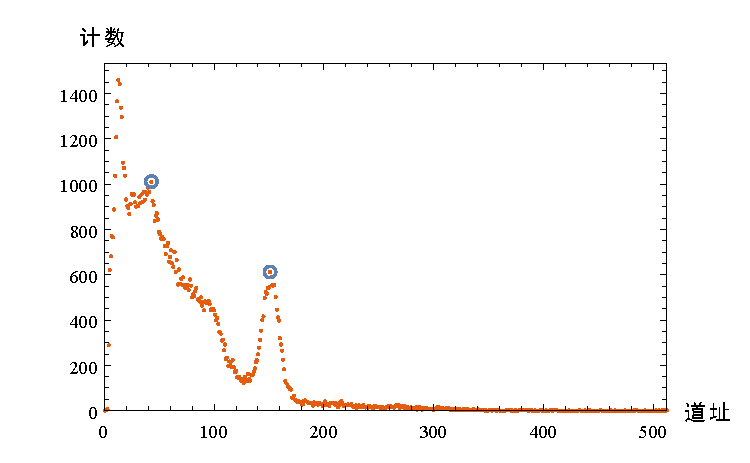
\includegraphics[width=.48\linewidth]{csPlot.pdf}	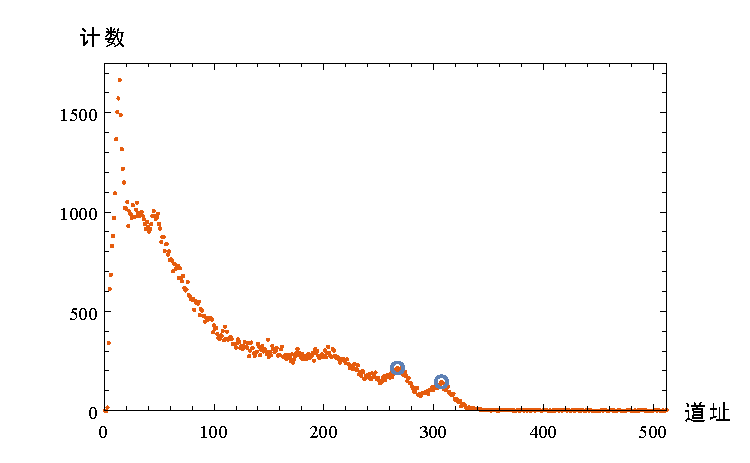
\includegraphics[width=.48\linewidth]{coPlot.pdf}
	\caption[探测器校准]{多道分析器的定标,\\
		左图为\CsAtom 能谱,右为\CoAtom 能谱,
		实际采样时长(活时)\SI{720}{\second}. \\
		标准峰值在图中以圆圈标出。}
	\end{figure}
\FloatBarrier

	测定标准源的能谱,结果如上;比较已知的\CsAtom 峰值(\SI{.662}{\MeV}, \SI{.184}{\MeV})和\CoAtom 峰值(\SI{1.173}{\MeV}, \SI{1.333}{\MeV}),可得线性关系\footnote{%
		简洁起见,此后的动能$E_k$均略去角标,记为$E$. }:
	\begin{equation}
	\begin{gathered}
		n = \pqty{
			(\num{.00(2)})
			+ (\num{2.29(2)})\cdot\frac{E}{\si{\MeV}}
			}\times\num{e2},\\
		R^2 = \num{,9998}
	\end{gathered}
	\end{equation}
	
	利用该式,即可由$n$得到$\beta$粒子的实测动能,进一步修正后得到真空室中$\beta$粒子的实际动能。在此基础上依次选取 \textnumero. \numrange{2}{8} 出射窗口,测定粒子的动能分布,如下所示;这里方便起见,依然选取道址作为能量的标度。
	
	\begin{figure}[!h]
	\centering
	\vspace{5ex}
	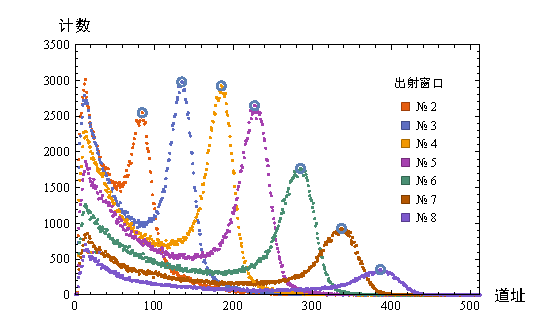
\includegraphics[width=\linewidth]{vacPlot.pdf}
	\caption[真空β能谱]{真空状态下探测到的$\beta$粒子的能谱,\\
	真空由机械泵抽取至极限获得,
	真空度$<\SI{-.1}{\MPa}$(相对大气压的压差)。\\
	能量由道址$n = 1,2,\dots,512$表征,峰值以圆圈标记。\\
	便于比较峰的强度,统一取活时 \SI{600}{\s}. }
	\label{fig:vacPlot}
	\end{figure}
	
	由图可见峰值及其强度随出射窗口的变化——出射窗口的编号越大,对应粒子运动半径$R$越大,即其动量$p$越大;相应地,峰值对应的道址$n$越大,即粒子的动能$E_k$越大。此外,能、动量增大,峰值的强度先增后减,这实际表征了\SrAtom--\Yatom\,$\beta$源的能谱。
	
	能谱峰值对应的道址由计算机获取,其不确定度通过具体分析峰值附近的图像确定;这一过程具体如图 \ref{fig:findPeaks} 所示。所得峰值道址$n$利用$n$--$E$关系转化为实测能量,再进一步修正得到$\beta$粒子能量;结果如表所示。
	
	\begin{figure}[p]
	\centering
	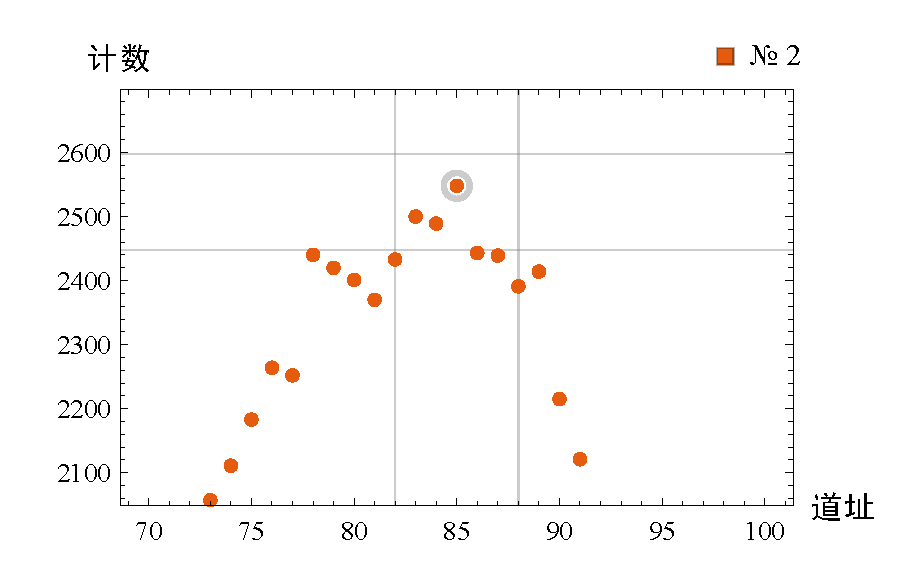
\includegraphics[width=.48\linewidth]{vacPeak2.pdf}	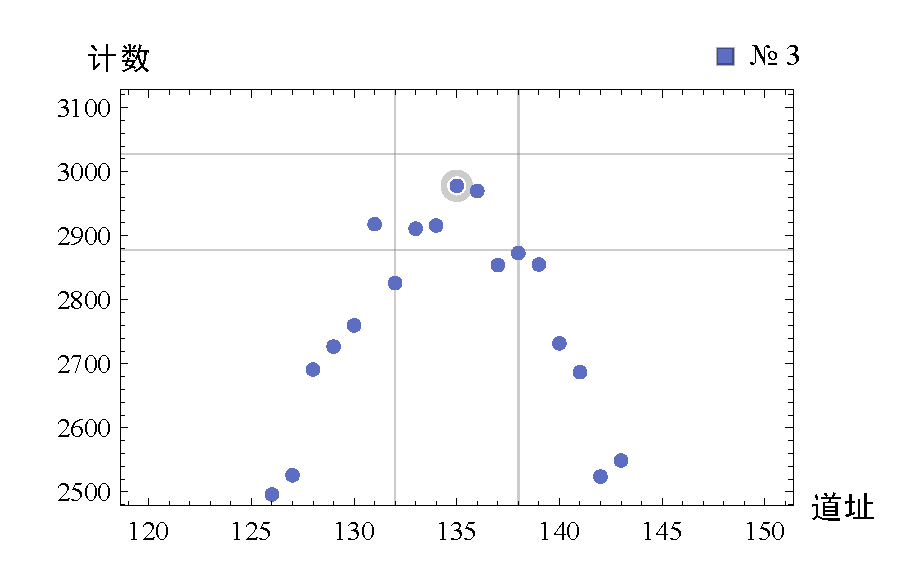
\includegraphics[width=.48\linewidth]{vacPeak3.pdf}	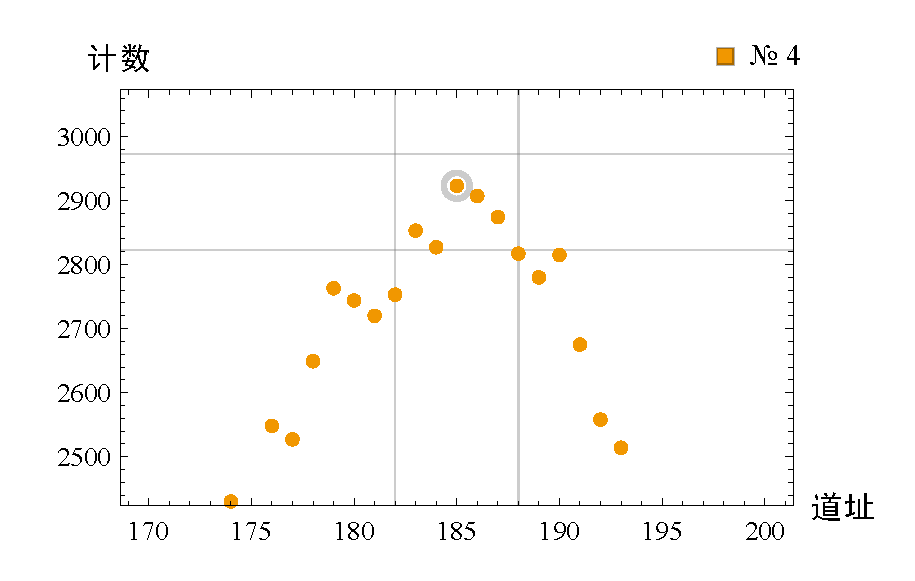
\includegraphics[width=.48\linewidth]{vacPeak4.pdf}	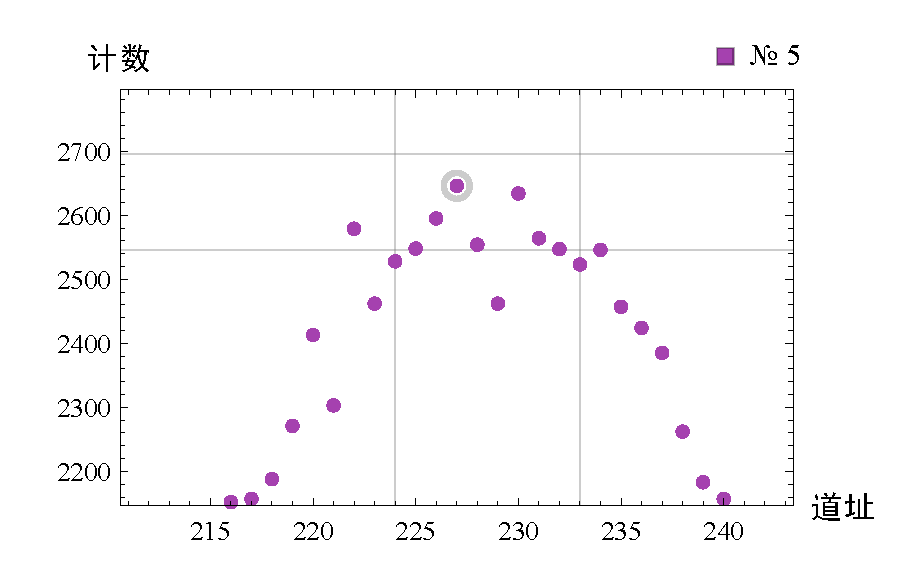
\includegraphics[width=.48\linewidth]{vacPeak5.pdf}	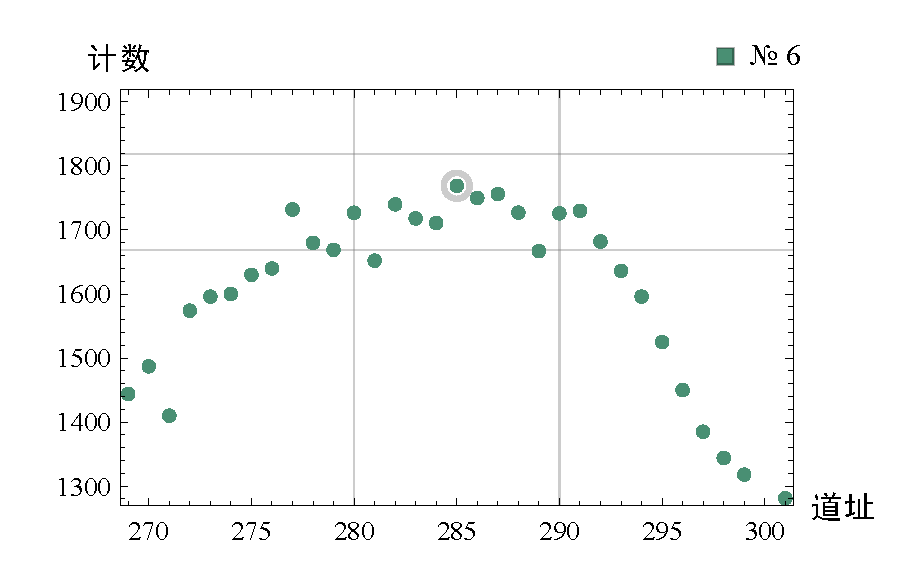
\includegraphics[width=.48\linewidth]{vacPeak6.pdf}	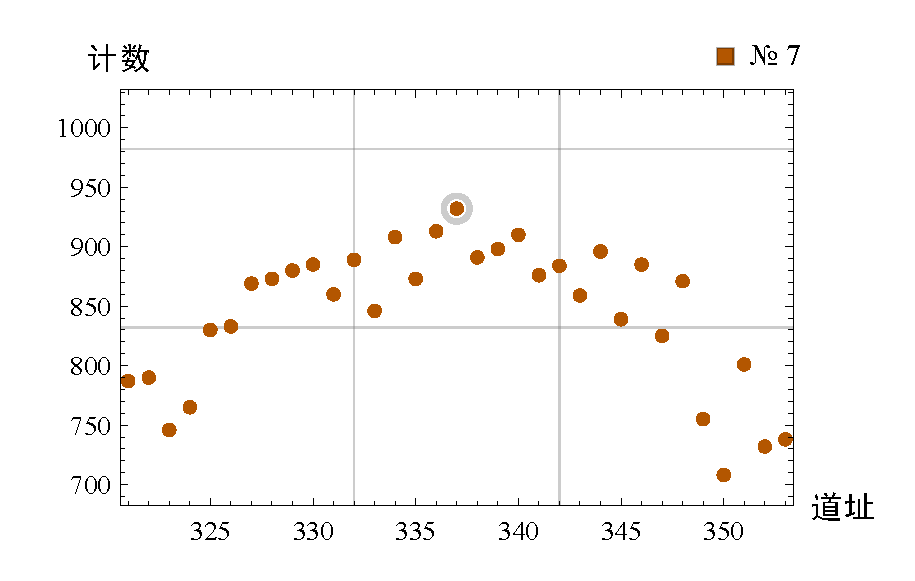
\includegraphics[width=.48\linewidth]{vacPeak7.pdf}	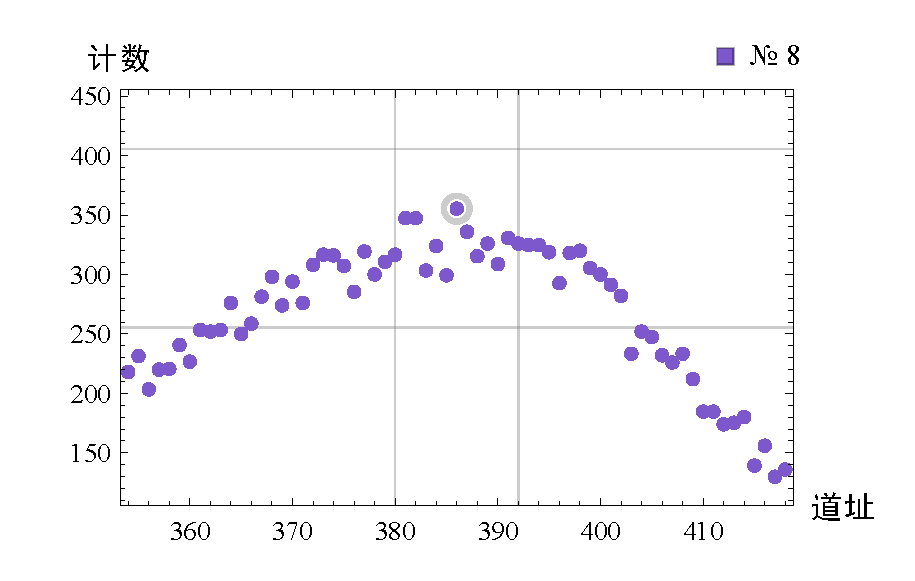
\includegraphics[width=.48\linewidth]{vacPeak8.pdf}
	\caption[真空β能谱峰值]{真空$\beta$能谱(图\ref{fig:vacPlot})峰值的局部放大,\\
	参考线表征峰值的极限不确定度。}
	\label{fig:findPeaks}
	\end{figure}
\FloatBarrier
	
	\begin{table}[!h]
	\caption[能量修正]{$\beta$粒子的能量测定数据表,\\
		道址不确定度由图 \ref{fig:findPeaks} 确定,
		实际能量由实测能量修正后得到。\\
		最终不确定度$\var{E}$包含了$\var{n}$及线性拟合的贡献。
		\textnumero 为出射窗口编号。}
	\centering\footnotesize
	\begin{tabularx}{.95\linewidth}{C{.2}C{.5}C{.8}*3{C{1}}}
	\toprule\midrule
    \textnumero &
    道址$n$ &
    不确定度$\var{n}$ &
    实测能量$\!/\si{\MeV}$ &
    实际能量$E/\si{\MeV}$ &
    不确定度$\var{E}/\si{\MeV}$  \\
    \midrule
		2     & 85    & 3     & 0.37  & 0.49  & 0.02 \\
		3     & 135   & 3     & 0.59  & 0.69  & 0.02 \\
		4     & 185   & 3     & 0.81  & 0.90  & 0.02 \\
		5     & 229   & 5     & 1.00  & 1.09  & 0.02 \\
		6     & 285   & 5     & 1.24  & 1.33  & 0.03 \\
		7     & 337   & 5     & 1.47  & 1.56  & 0.03 \\
		8     & 386   & 6     & 1.69  & 1.78  & 0.03 \\
    \midrule\bottomrule
	\end{tabularx}
	\end{table}
\FloatBarrier
	
	在此基础上,将$E$--$p$关系作图如下;其中,$p = eBR$的误差主要由$R$即$x$测定时的误差导致,由于刻线不甚精确,估计$\var{x}$的上限高达 \SI{1}{\mm}. 
	\begin{figure}[!h]
	\centering
	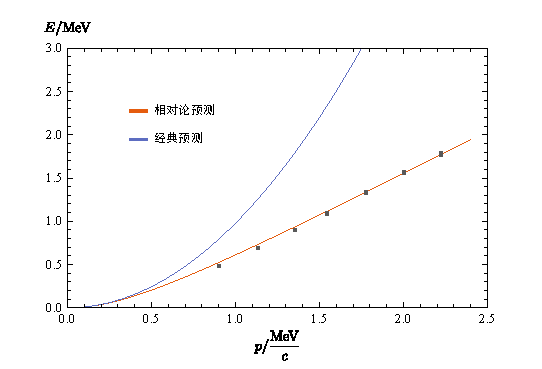
\includegraphics[width=.9\linewidth]{epRelations.pdf}
	\caption[色散关系]{$\beta$粒子的动量--能量关系,
		理论预测由曲线给出。\\
		实测数据表现为图中散点,散点的尺度体现了其不确定度。}
	\end{figure}
\FloatBarrier
	
	可见,实测数据与相对论性结果吻合得非常好,同时与经典结论明显不符。这便证实了高能$\beta$粒子遵循相对论性动量--能量关系。
	
	\newparagraph
	进一步,考察空气对粒子运动的影响。在 \SI{1}{atm} 下重复实验,比较能量分布曲线,所得结果如下。可见,空气环境使峰值位置向道址更低方向(低能方向)偏移,且对峰值强度的影响十分明显;由于能量分布变得平缓,峰值位置的不确定度显著增大,这也不利于精确测定粒子的动能。
	
	\begin{figure}[!h]
	\centering
	\centering
	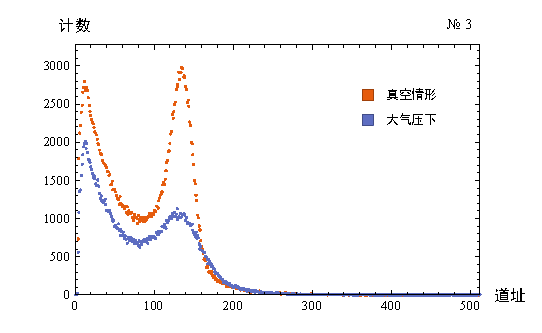
\includegraphics[width=.48\linewidth]{vacAirCompare3.pdf}
	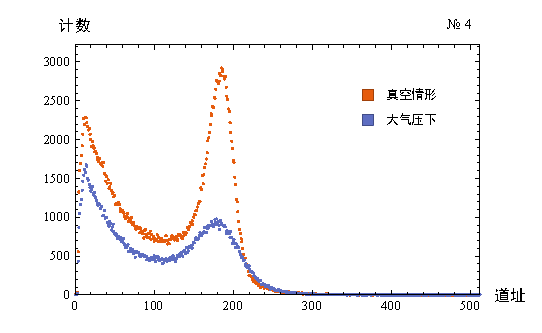
\includegraphics[width=.48\linewidth]{vacAirCompare4.pdf}
	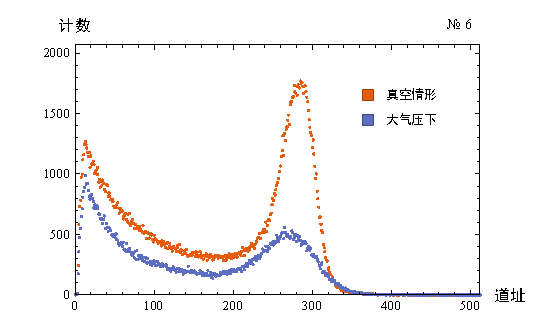
\includegraphics[width=.48\linewidth]{vacAirCompare6.pdf}
	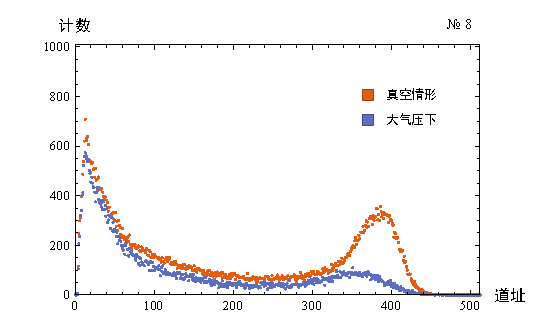
\includegraphics[width=.48\linewidth]{vacAirCompare8.pdf}
	\caption[大气情形]{真空与 \SI{1}{atm} 下$\beta$能谱的比较}
	\label{fig:vacAirComp}
	\end{figure}
	
	在此基础上,我们尝试估计$\beta$粒子在$\SI{1}{atm}$的\textit{衰减长度}$L_0$. 与空气分子的碰撞导致沿轨迹运动的粒子数目指数衰减,考虑探测装置的效率$\epsilon$, 有探测到的粒子数目:
	\begin{equation}
		N_0 = \epsilon C\,e^{-\frac{L}{L_0}},\quad
		p = p_0 = \SI{1}{atm}
	\end{equation}
	
	此外,粒子的自由程反比于压强,故改变压强$p$时,有:
	\begin{equation}
		N = \epsilon C\,e^{-\frac{pL}{p_0 L_0}}\quad
		\Longrightarrow\quad
		L_0 = L\pqty{1 - \frac{p}{p_0}} \bigg/ \ln\frac{N}{N_0}
	\end{equation}
	本实验中,$L = \pi R,\,\pqty\big{1 - \frac{p}{p_0}} \to 1$, 进一步有:
	\begin{equation}
		L_0 = \pi R \bigg/ \ln\frac{N}{N_0}
	\end{equation}
	
	考虑本实验测得的能谱,如图 \ref{fig:vacAirComp} 所示,实际上只有构成峰值的粒子是沿$L = \pi R$路径抵达探测器的,峰值以外的能谱是被散射后的粒子之贡献,在能谱上体现为一指数衰减的背景。在计数$N$值时,应当去除这一背景;去除的方法如图所示。
	\begin{figure}[!h]
	\centering
	\centering
	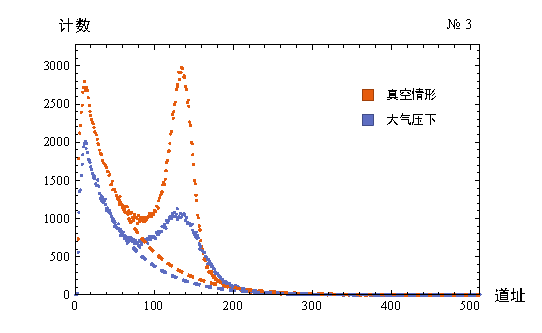
\includegraphics[width=.48\linewidth]{plotBgRemoved3.pdf}
	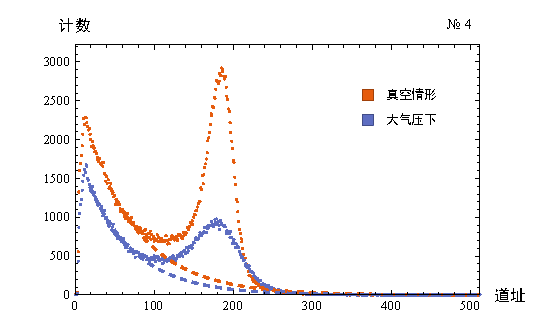
\includegraphics[width=.48\linewidth]{plotBgRemoved4.pdf}
	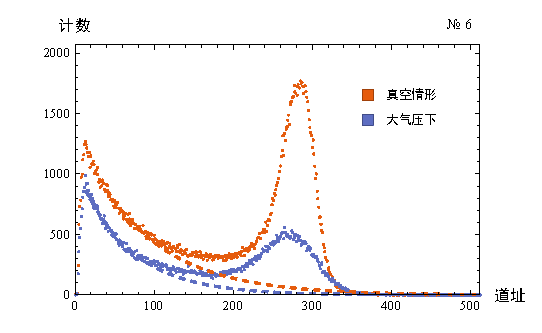
\includegraphics[width=.48\linewidth]{plotBgRemoved6.pdf}
	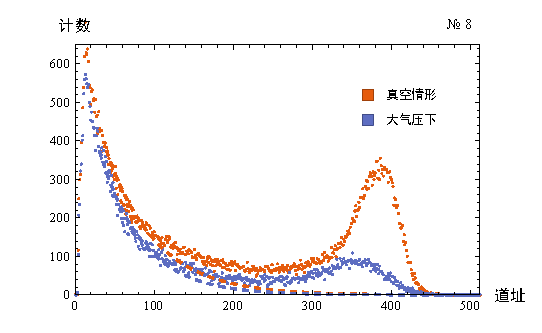
\includegraphics[width=.48\linewidth]{plotBgRemoved8.pdf}
	\caption[背景除去]{背景能谱的识别与去除,以指数衰减的曲线表示。\\
		注意到背景能谱的拟合实际上有不小的自由度;\\
		尤其对于 \textnumero. 8 的情形,峰值展宽太大,难以精确拟合。\\
		故由此计算得到的结果仅作为$L_0$的一个估计值。}
	\label{fig:bgRemoved}
	\end{figure}
\pagebreak
	
	\begin{table}[!h]
	\caption[衰减长度]{$\beta$粒子在 \SI{1}{atm} 空气中的衰减长度$L_0$测定,\\
		由于$N,N_0$的不确定度很大,这里的计算仅作为$L_0$的一个估计。\\
		\textnumero 为出射窗口编号。}
	\centering\footnotesize
	\begin{tabularx}{.75\linewidth}{C{.5}*2{C{1}}C{.8}C{1}}
    \toprule\midrule
		\textnumero &
		$N$ &
		$N_0$ &
		$R/\si{cm}$ &
		$L_0/\si{cm}$  \\
    \midrule
		3     & 111308 & 59190 & 6.3   & 31.3 \\
		4     & 131269 & 65565 & 7.5   & 33.9 \\
		6     & 107650 & 45078 & 9.8   & 35.4 \\
    \midrule\bottomrule
	\end{tabularx}
	\end{table}
	
	可见,$\beta$粒子在空气中的衰减长度$L_0$大致为三十几厘米,且$L_0$似乎随着粒子能动量(对应出射窗口编号)的增大而增大。
	
	当然,由于实际测算的数据只有3组,这一结论的置信度并不很高,需要进一步实验加以证实;但可以肯定的是,该能量范围的$\beta$粒子在 \SI{1}{atm} 下的衰减长度大致均在 \SIrange{30}{40}{cm} 上下,与$L$在同一量级。这也进一步肯定了在真空环境中进行实验的必要性。
\section{结论}
%%%	首先要给出实验结果,然后再给出由实验结果分析得到的结果和结论.此部分给出的内容要比摘要中的全面,用词要更准确.\par
%%%%%%%%%%%%%%%%%%%%%%%%%%%%%%%
	实验证实了高能$\beta$粒子的动量--动能的关系(色散关系)满足狭义相对论的理论预测,即在误差容许的范围内,有:
	\begin{equation}
		E_k = \sqrt{p^2 c^2 + m^2 c^4} - m^2 c^4
		\tag{\ref{eq:relativityEk}}
	\end{equation}
	从而初步验证了狭义相对论对高速运动物体的适用性。同时,实验结果与经典理论的严重偏离确认了经典力学对高速运动不适用。
	
	在此基础上,实验估测了$\beta$粒子在 \SI{1}{atm} 空气中的衰减长度$L_0 \sim \SIrange{30}{40}{cm}$, 从而强调了真空环境对提高数据质量的重要意义。此外,观察到衰减长度$L_0$似乎随着粒子能量增大而增大,这一结论符合直观;但由于数据量有限,需要进一步的实验加以确认。
\section{致谢}
%	此部分感谢同组人...和对实验和报告有帮助的人.
%%%%%%%%%%%%%%%%%%%%%%%%%%%%%%
	亲手接触放射源,还是有一些紧张的;感谢同组的韩霄同学,我们的讨论成果保证了实验顺利进行并获得成功。也感谢王思广老师细致而耐心的指导,这给我们带来了巨大的帮助。

\setlength{\bibsep}{2pt}
\linespread{1.2}\selectfont
\bibliographystyle{../BibStyle/gbt-7714-2015-numerical}
\bibliography{../BibStyle/Textbook,bib/Ref}

\clearpage
\end{document}
